%!TEX root = /Users/zolkko/Projects/zolkko-alarm/doc/main.tex
\subsection{Разработка принципиальной электрической схемы управляющего устройства в системе Eagle}
Для создания принципиальных электрических схем в системе Eagle используется программа
Eagle Layout Editor (рисунок \ref{img:schemeEd}).
\begin{figure}[ht]
	\center{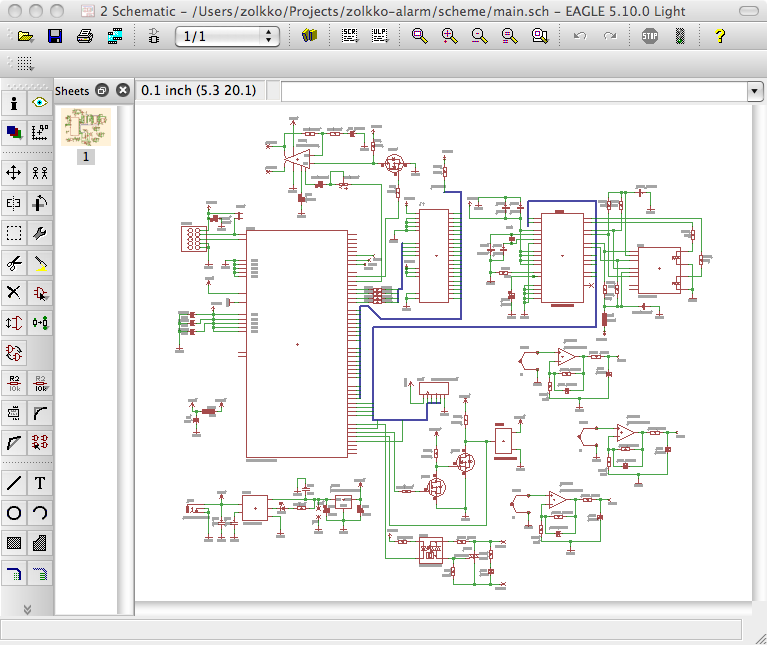
\includegraphics[bb=0 0 767 645, clip, scale=0.5]{scheme_ed.png}}
	\caption{Окно редактора Eagle Layout Editor}
	\label{img:schemeEd}
\end{figure}

Чтобы открыть новое окно Eagle Layout Editor нужно вызвать команду ''Schematic''
главного меню ''New''. Эта программа, по своей сути, является программой используемой раннее для создания
символов для пользовательской библиотеки.

Однако, в отличии от редактора топологических схем, в редакторе принципиальных схем не рекомендуется при проведении
начальной конфигурации системы менять значения шага сетки. Так как если задать не правильное
значение шага сетки командой ''Grid'', то в последующем будет невозможно соединить выводы
компонентов стандартной библиотеки соединительными линиями. Если из-за ошибочного действия или необходимости
использовать компонент с нестандартным шагом выводов размер шага сетки всё же был изменён, то вернуть его в
начальное состояние помжно нажав на кнопку ''Default'' диалога ''Grid'' (рисунок \ref{img:gridDlg}).
\begin{figure}[ht]
	\center{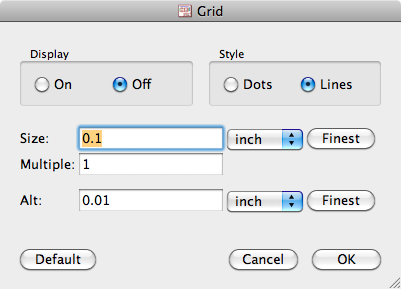
\includegraphics[bb=0 0 401 289, clip, scale=0.5]{grid_dlg.png}}
	\caption{Диалоговое окно ''Grid''}
	\label{img:gridDlg}
\end{figure}


\subsubsection{Ввод принципиальной электрической схемы}
Инсталляционный пакет программы Eagle как Lite, так и Professional версий помимо самой программы, так же
содержит обширный перечень библиотек компонентов. При  запуске программы все стандартные библиотеки подключаются
к системе, так что их можно использовать не производя дополнительных действий.


Однако, так как в схеме управляющего устройства предполагается использовать компоненты созданной,
пользовательской библиотеки, то её предварительно необходимо добавить в список используемых библиотек.

Дл этого необходимо вызвать команду ''Use'' главного меню ''Library'' и в диалоговом окне открытия файла
указать место расположения пользовательской библиотеки.


Добавление новых символов на схему осуществляется командой ''Add''. Выполнение этой команды приводит к
выводу на экран диалогового окна добавления нового компонента (рисунок \ref{img:addDlg}).
\begin{figure}[ht]
	\center{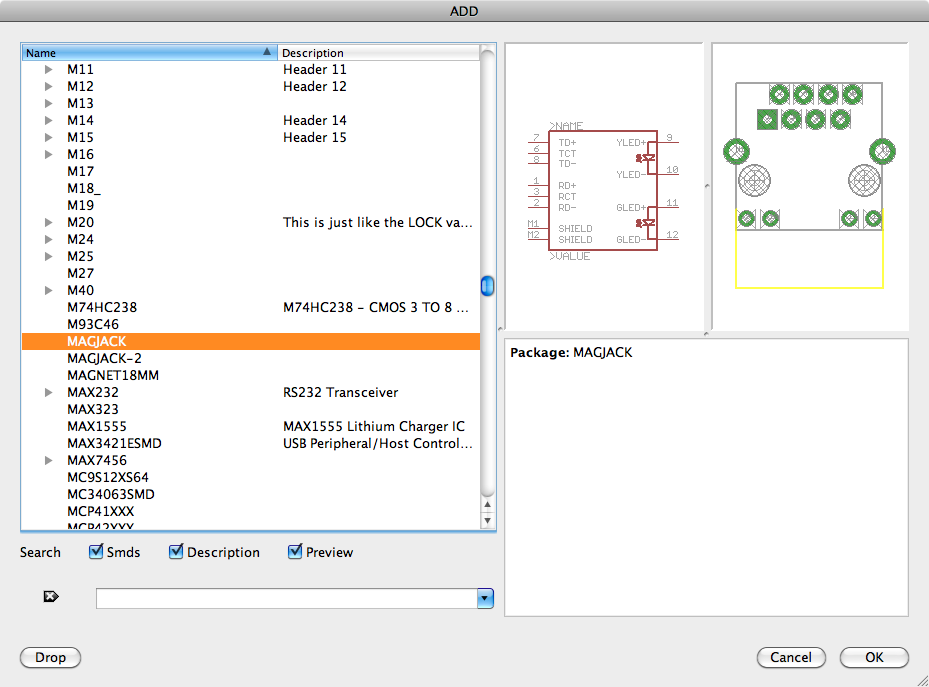
\includegraphics[bb=0 0 929 687, clip, scale=0.3]{add_dlg.png}}
	\caption{Диалоговое окно ''Add''}
	\label{img:addDlg}
\end{figure}

В этом диалоге можно либо в ручную выбрать необходимый компонент из списка, либо воспользоваться строкой поиска.
Маскирование строки поиска компонента выполняется символом ''*''.


Помимо стандартных команд и инструментов таких как ''move'', ''copy'', ''paste'', ''rotate'',
редактор принципиальных электрических схем имеет ряд команд специфичных только для этого
режима работы программы.

Наиболее важными из них являются две.
\begin{par}
 	1.	''invoke'' -- позволяет выбрать конкретный символ используемого устройства. В частности
	только используя эту команду на принципиальную схему возможно ввести символ обозначающий линии
	питания много-компонентной микросхемы ad8544. После ввода этой команды и выбора на схеме 
	много-компонентного устройства, на экран будет выведено диалоговое окно добавления компонента
	(рисунок \ref{img:addGateDlg}).
	
	\begin{figure}[ht]
		\center{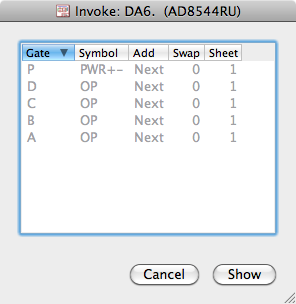
\includegraphics[bb=0 0 296 304, clip, scale=0.8]{invoke_dlg.png}}
		\caption{Диалоговое ''Invoke''}
		\label{img:addGateDlg}
	\end{figure}
\end{par}
	
\begin{par}
 	2.	''bus'' -- позволяет вводить шины на принципиальной схеме. Примером такой шины является
		соединение микросхемы enc28j60, микроконтроллера и слота SSD.
		Сигналы проходящие пошине определяются её название.
		Для этого необходимо либо используя инструмент ''info'', либо инструмент ''name'' ввести
		текстовое значение -- список сигналов. Сигналы в строке должны отделяться друг от друга
		символом '',''. Если нужно ввести массив сигналов, то диапазон массива указывается в
		квадратных скобках, где начало и конец диапазона разделены строкой ''..''. Например
		название шины ''SS,AS[0..2]'' определяется 3 сигнала: ''SS'', ''AS0'', ''AS1'', ''AS2''.
		
		Подключение выводов компонентов к шине производиться с использованием инструмента ''Net''.
		При этом на экран выводиться выпадающий список сигналов на выбор.
\end{par}


Результатом проделанной работы стала схема электрическая принципиальная,
представленная в приложении Б.


\subsubsection{Принцип работы схемы управления датчиком температуры холодного спая}
Для получение температуры холодного спая в устройстве управления используется цифровой датчик
температуры общего применения DS18B20.

Данный датчик работает по протоколу 1-wire -- минималистичный интерфейс, использующий
всего одну линию для передачи данных. Обычно в качестве ведущего устройства
шины 1-wire используют один выводов микроконтроллера, а для формирования
тайм-слотов необходимой длительности -- применяют либо задержки сформированные
командами NOP, либо пустыми циклами.


Однако, для формирования тайм-слотов такими способами, на высоких рабочих
частотах, микроконтроллер использует слишком большое количество машинных циклов.


Для решения этой проблемы компания Maxim Integrated Products Inc.
предлагает использовать \cite{max2usart} свободный модуль UART микроконтроллера.


Сконфигурировав модуль UART по схеме 8 бит данных, без чётности, один стоп-бит и
манипулируя скоростью передачи, его можно использовать для формирования
импульсов нужной длинны.


В шине 1-wire ведомое устройство для ответа должно иметь возможность
опускать или оставлять не именным уровень логической единицы,
передаваемый ведущим.
Однако, вывод TX модуля UART, фактически замкнутый на его же вход RX у большинства
микроконтроллеров не является выводом с общим коллектором, а значит и ведомое
устройство не сможет опустить шину до уровня логической единицы.

Для решения этой проблемы, в цепь TX перед первым ведомым устройством, внедряется
буферная схема с общим коллектором.

В схеме устройства управления, в качестве такого не инвертирующего буферного
элемента c общим стоком мной используются два полевых NPN транзистора с изолированным
затвором -- 2N7002.

Номиналы подтягивающих резисторов в цепи тока и цепи затвора транзисторов брались из расчёта:
\begin{itemize}
	\item максимальный ток DS18B20 -- 5 мА;
	\item максимальный ток 2N7002 -- 115 мА;
	\item максимальный ток вывода ATXMega -- 150 мА;
	\item минимальный уровень логической единицы при напряжении
		питания микроконтроллера 3.3 В -- 0.8 В.
\end{itemize}
Этим условиям удовлетворяют сопротивления номиналом 2.7 KОм.


\subsubsection{Расчёт параметров элементов схемы усиления сигнала термопары}
Сигналы от термопары принимают значения от микровольт до милливольт, поэтому необходимо принимать
дополнительные меры по снижению уровня шумов и наводок.
Обычно это экранирование и сокращение длины соединительных проводов.

Кроме того, учитывая, что термоэдс термопары в процессе её работы изменяется
с низкой частотой, можно подавлять помехи с помощью
фильтра нижних частот. В устройстве управления такие фильтры устанавливаются на выходах
каждого усилителя сигнала термопар.

Для упрощения схемы, устройства в ней используется фильтр нижих частот первого порядка, с
частотой среза 2 Гц и желаемой граничной частотой полосы задержания 4 Гц на 50 бД.

\begin{equation}
	F = \frac{1} {2 \times{} \pi{} RC}
\end{equation}

Соответственно при сопротивлении  $R = 1500$ \\
$C = \frac{1}{2\pi{}R} = \frac{1}{1500 \times{} 6.28} = 0.0001$ Ф.

\subsubsection{Управление светодиодной подсветкой ЖКИ DST2001PH}
Одним из основных параметров светодиодов является: яркость -- величина,
равная отношению силы света к площади светящейся
поверхности, измеряемая в канделах на квадратный метр.

Спектральная характеристика светодиода выражает зависимость интенсивности
излучения от длины волны излучаемого света и дает представление о цвете
свечения светодиода.


Длина волны излучаемого света определяется разностью
энергий двух энергетических уровней, между которыми происходит переход
электронов на излучательном этапе процесса рекомбинации и определяется
исходным полупроводниковым материалом и легирующими примесями.

% http://www.e-neon.ru/user_img/pages/Dimming_InGaN_rus.pdf
Наиболее простой способ уменьшения яркости светодиода - изменение прямого
тока или напряжения. Но необходимо учитывать, что изменение этих параметров будет
влиять на длину волны излучаемого света, причём чем больше длинна волны, тем сильнее
выражен этот эффект. Помимо тока, на длину волны оказывает влияние так же и температура.
Но это влияние не столь существенно и может игнорироваться.


В схемах с использованием ШИМ управление через светодиод проходит последовательность импульсов.
Если частота следования импульсов более 200 Гц, человеческий глаз, обладающий инерционностью,
будет ощущать непрерывное свечение светодиода. Изменняя длительность и скважность импульса
можно добиться того, что зрение будет интегрировать и интерпретировать отдельные световые
импульсы как изменение силы света (рисунок \ref{img:ledpwm}).


\begin{figure}[H]
	\center{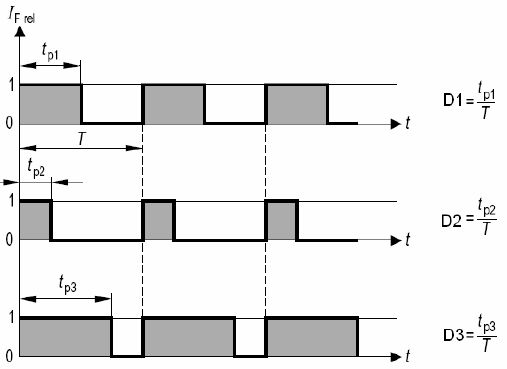
\includegraphics[bb=0 0 450 270, clip, scale=0.9]{led_pwm.png}}
	\caption{Управление яркосьтю светодиода ШИМ}
	\label{img:ledpwm}
\end{figure}


При неизменном токе яркость свечения зависит от скважности
следующим образом: $D_2 < D_1 < D_3$.

При этом, визуальная сила света будет меняться линейно при соответствующем
линейном изменении скважности.

В ГЖКИ DST2001PH используются четыре параллельно соединённых светодиода белого
свечения со следующими характеристиками:
\begin{itemize}
    \item{}допустимый ток --- 15 мА;
    \item{}прямое падение напряжения --- 3.2 В.
\end{itemize}

Таким образом ограничивающий ток резистор должен иметь сопротивление не менее
$R = \frac{U_n - U_p}{I} = \frac{3.3 - 3.2} {0.015} = 6.6$ Ом.
Ближайшее значение стандартного резистра будет 6.8 Ом.
